\documentclass{beamer}
\mode<presentation> {
	\usetheme{Copenhagen}
	% remove the navigation symbols from the bottom of all slides
	\setbeamertemplate{navigation symbols}{}
}

\usepackage[T1]{fontenc}
\usepackage[utf8]{inputenc}
\usepackage{lmodern}
\usepackage{float}
\usepackage{enumerate, enumitem}
\usepackage{graphicx}
\usepackage{microtype}
\usepackage{mathtools}
\usepackage{amssymb,amsmath}
\usepackage{listings}
\usepackage{media9, xcolor}
\usepackage{biblatex}
\usepackage{hyperref}

\addbibresource{bib.bib}

\lstset{columns=fullflexible}
\newcommand{\link}[1]{{\color{blue}\href{#1}{#1}}}

\title{In-vehicle baby alert system}
\subtitle{Advanced Digital Image Processing project}
\author{F. Casciola, E. G. Ceroni, N. Landolfi} %ordine alfabetico
\institute[Unisi]{Università degli Studi di Siena}
\date{date TBD}

%Per poter compilare le slides con TexStudio, verificare che:
%1. Options - Configure TexStudio - Commands - Biber sia uguale a `biber.exe %`
%2. Options - Configure TexStudio - Build - Default Biblio Tool sia uguale a `Biber`

\begin{document}
	
	
	\begin{frame}
		\frametitle{Child-seat Detection system}
		When used properly, only children should be sitting on the child-seat. This assumption would imply a completely different approach for the detection of the presence of the child in the car. 
		
\bigskip		
		Instead of relying on the face detection and classification, we can assume that, when a child seat is detected in a certain region, if a face is detected in the same region that would belong to a child. Under this assumption it would be possible to perform the face classification task fewer times in order to increase the general speed of  the system.
		
	\end{frame}	
	
	\begin{frame}
		\frametitle{Child-seat Detection system}

		In order to find the region where the child-seat is, we decided to employ SIFT descriptors in order to store features from the child seat owned by the user and use them to recognise future instances of the same. 
		
		\bigskip
		The collection of the SIFT descriptors would be performed through the same camera used for the detection in order to ensure little variation in the point of view over the cild-seat. The collection of the descriptors is bound to the presence of the child-seat, therefore the system must include a detector for a generic child-seat. 
		
	\end{frame}	
	
	\begin{frame}
		\frametitle{Child-seat Detection system}
		\begin{figure}
			\centering
			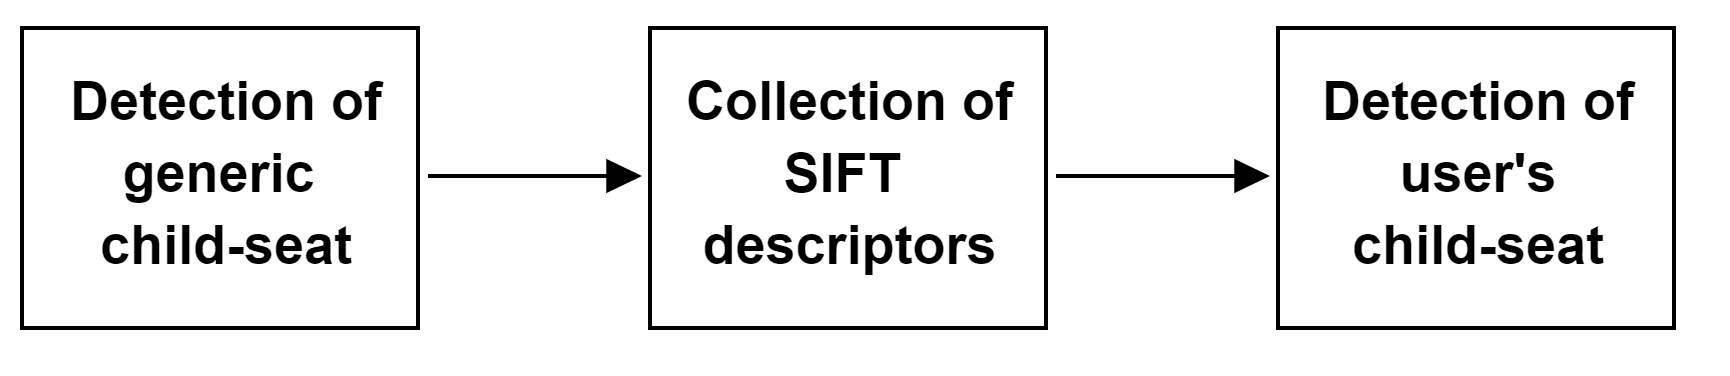
\includegraphics[width=0.7\textwidth]{img/SIFT_collection.png}
		\end{figure}
		The steps for our generic child seat detection system are:
		\begin{enumerate}[leftmargin=*, label={\textbf{Step \arabic*}}: , ref={\textbf{Step \arabic*}}]
		\item Collection of SIFT descriptors from child-seat pictures.
		\item Creation of a Bag Of Visual Words $\mathcal{B}$ using KMeans clustering algorithm
		\item Collection of SIFT descriptors from the camera input and representation in the BOVW feature space
		\item We assume that the input $\hat{x}$ contains a child seat if the following statement holds true for at least $n$ patterns in $\mathcal{B}$:
		\begin{equation*}
		\mid\mid\hat{x}-x_B\mid\mid<\gamma\, ,\quad x_B\in \mathcal{B}
		\end{equation*}
		
		\end{enumerate} 
		
	\end{frame}	
	
	\begin{frame}
		\frametitle{Generic Child Seat Detection}
		Using $275$ pictures gathered from the internet, $50$ clusters when creating the BOVW and as parameters $n=10, \gamma=0.1$, we obtained the following result:
		
		\bigskip
		\begin{minipage}{0.5\textwidth}
		\begin{center}
		{\small Input frames}
		\end{center}
		\end{minipage}%
		\begin{minipage}{0.5\textwidth}
		\begin{center}
		\begin{small}
		Frames where a child-seat\
		has been detected
		\end{small}
		\end{center}
		\end{minipage}
		
		\bigskip
		\includemedia[
		width=\textwidth,
		addresource=videos/detection.mp4,
		transparent,
		activate=pagevisible,
		flashvars={
		source=videos/detection.mp4
		&autoplay=true
		&loop=false}
		]
		{\textcolor{white}{Video}}{VPlayer9.swf}
	\end{frame}
	
	\begin{frame}
		\frametitle{User's Cild-seat Detection}

From the frames where a generic child-seat is detected the SIFT descriptors are computed. 

\bigskip
Ideally, if the car's backseat is free from clutter, the descriptors should gather around the child-seat. A good way to remove decriptors not belonging to the cild-seat, would be to use the mean and standard deviation of the key-points' position to exclude the outliers. 

\bigskip
The detection of the user's child seat is performed by comparing the SIFT descriptors gathered in the previous step with the new ones from the camera input.
		
	\end{frame}
	
	
	\begin{frame}
		\frametitle{User's Child Seat Detection}
		Using two frames (and their horizontally flipped versions) from the unprocessed version of the video below, we obtained the following result. 
			
		\bigskip
		\includemedia[
		width=\textwidth,
		addresource=videos/BB.mp4,
		transparent,
		activate=pagevisible,
		flashvars={
		source=videos/BB.mp4
		&autoplay=true
		&loop=false}
		]
		{\textcolor{white}{Video}}{VPlayer9.swf}
		
		\bigskip
		The red circle is the mean of the key-points (black circles), the green bounding box includes all the keypoints while the blue one is a $200$x$200$ pixels square centered in the mean. 
	\end{frame}

\end{document}

